\begin{center}
    \begin{large}
    Cp 4 - Ciclos\\
    Curso \academicyear\\
    \end{large}
    \begin{figure}[h]
    	\centering
    	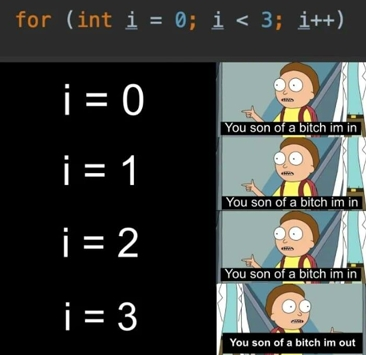
\includegraphics[width=0.5\linewidth]{cp4/loops.jpg}
    \end{figure}
\end{center}

\section{Factorial}
El factorial de un número $n$ (denotado como $n!$) se define como el producto de todos los números enteros positivos desde 1 hasta $n$, o sea:

\[
n! = \prod_{k=1}^{n} k
\]

o lo que es lo mismo:

\[
n! =
\begin{cases} 
1 & \text{si } n = 0 \\
n \cdot (n-1)! & \text{si } n > 0
\end{cases}
\]

Implemente un programa que reciba un número entero no negativo \(n\) de la consola y calcule el factorial de ese número.

\subsection*{Ejemplos:}
\begin{itemize}
    \item Entrada: \texttt{0}\\
          Salida: \texttt{El factorial de 0 es 1.}
    \item Entrada: \texttt{1}\\
          Salida: \texttt{El factorial de 1 es 1.}
    \item Entrada: \texttt{5}\\
          Salida: \texttt{El factorial de 5 es 120.}
    \item Entrada: \texttt{7}\\
          Salida: \texttt{El factorial de 7 es 5040.}
\end{itemize}


\ifshowanswers
\section*{Respuesta:}
\begin{lstlisting}
public static long CalculateFactorial(int n)
{
    long result = 1;
    
    for (int i = 1; i <= n; i++)
    {
        result *= i;
    }
    
    return result;
}
\end{lstlisting}
\fi

\section{Suma de impares}
Implemente un programa que reciba un entero \(n\) e imprima la suma de los primeros \(n\) números impares.

Formalmente, los números impares son aquellos de la forma \(2k + 1\), donde \(k \in \mathbb{Z}_{\geq 0}\). La suma de los primeros \(n\) números impares se puede expresar como:

\[
S_n = \sum_{k=0}^{n-1} (2k + 1).
\]

\subsection*{Ejemplos}
\begin{itemize}
    \item Entrada: \texttt{1}\\
          Salida: \texttt{La suma de los primeros 1 números impares es 1.}
    \item Entrada: \texttt{3}\\
          Salida: \texttt{La suma de los primeros 3 números impares es 9.}
    \item Entrada: \texttt{5}\\
          Salida: \texttt{La suma de los primeros 5 números impares es 25.}
    \item Entrada: \texttt{7}\\
          Salida: \texttt{La suma de los primeros 7 números impares es 49.}
\end{itemize}


\ifshowanswers
\section*{Respuesta:}
\begin{lstlisting}
public static int SumOddNumbers(int n)
{
    int sum = 0;
    
    for (int i = 1; i < 2 * n; i += 2)
    {
        sum += i;
    }
    
    return sum;
}
\end{lstlisting}

Este código usa un ciclo para sumar los primeros \(n\) números impares. Sin embargo, podemos notar una propiedad interesante (que puedes demostrar por inducción):
\[
1 + 3 + 5 + \ldots + (2n-1) = n^2
\]
Por lo tanto, podemos optimizar nuestro código utilizando esta propiedad matemática.

\begin{lstlisting}
public static int SumOddNumbers(int n)
{
    return n * n;
}
\end{lstlisting}
\fi

\section{Mayor, menor y promedio de forma perezosa}
Implemente un programa que lea una secuencia de números de la consola (uno por línea) hasta que se escriba una línea en blanco y de estos imprimir:
\begin{itemize}
    \item El mayor
    \item El menor
    \item Su promedio
\end{itemize}

\subsection*{Ejemplos}
\begin{itemize}
    \item Entrada:
\begin{verbatim}
12
8
15
22
5
(línea en blanco)
\end{verbatim}
    Salida:
\begin{verbatim}
El mayor número es: 22
El menor número es: 5
El promedio es: 12.4
\end{verbatim}

    \item Entrada:
\begin{verbatim}
3
3
3
(línea en blanco)
\end{verbatim}
    Salida:
\begin{verbatim}
El mayor número es: 3
El menor número es: 3
El promedio es: 3.0
\end{verbatim}
\end{itemize}


\ifshowanswers
\section*{Respuesta:}
\begin{lstlisting}
string input;
int max = int.MinValue;
int min = int.MaxValue;
int sum = 0;
int count = 0;
Console.WriteLine("Introduce números enteros (deja la línea en blanco para finalizar):");

while (!string.IsNullOrWhiteSpace(input = Console.ReadLine()))
{
    if (int.TryParse(input, out int number))
    {
        if (number > max) max = number;
        if (number < min) min = number;
        sum += number;
        count++;
    }
    else
    {
        Console.WriteLine("Entrada inválida, introduce un número entero.");
    }
}
    
if (count == 0)
{
    Console.WriteLine("No se introdujeron números.");
}
else
{
    double average = (double)sum / count;

    Console.WriteLine($"El mayor: {max}");
    Console.WriteLine($"El menor: {min}");
    Console.WriteLine($"El promedio: {average}");
}
\end{lstlisting}
\fi

\section{Recorriendo arrays}
Implemente un método para cada inciso, que reciba un array de enteros y devuelva:
\begin{enumerate}[label=\alph*)]
    \item El mayor elemento de un array.
    \item El segundo menor elemento de un array.
    \item Si un número \(n\) pertenece al array \(a\).
    \item La posición de un número \(n\) en el array. Devuelve -1 si no aparece.
    \item El promedio de todos los elementos de un array.
    \item La cantidad de elementos que son mayor que el promedio en un array.
\end{enumerate}

\ifshowanswers
\section*{Respuesta:}
\begin{enumerate}[label=\alph*)]
    \item El mayor elemento de un array.
    \begin{lstlisting}
    public static int FindMax(int[] array)
    {
        int max = int.MinValue;
        
        for (int i = 0; i < array.Length; i++)
        {
            var num = array[i];
            if (num > max) max = num;
        }

        return max;
    }
    \end{lstlisting}
    \item El segundo menor elemento de un array.
    \begin{lstlisting}
    public static int FindSecondMin(int[] array)
    {
        int min = int.MaxValue;
        int secondMin = int.MaxValue;
        
        for (int i = 0; i < array.Length; i++)
        {
            int num = array[i];
            if (num < min)
            {
                secondMin = min;
                min = num;
            }
            else if (num < secondMin && num != min)
            {
                secondMin = num;
            }
        }

        return secondMin;
    }
    \end{lstlisting}
    \item Si un número \(n\) pertenece al array \(a\).
    \begin{lstlisting}
    public static bool Contains(int[] array, int n)
    {
        for (int i = 0; i < array.Length; i++)
        {
            int num = array[i];
            if (num == n)
                return true;
        }

        return false;
    }
    \end{lstlisting}
    \item El promedio de todos los elementos de un array.
    \begin{lstlisting}
    public static double CalculateAverage(int[] array)
    {
        int sum = 0;
        for (int i = 0; i < array.Length; i++)
        {
            sum += array[i];
        }

        return (double)sum / array.Length;
    }
    \end{lstlisting}
    \item La cantidad de elementos que son mayor que el promedio en un array.
    \begin{lstlisting}
    public static int CountAboveAverage(int[] array)
    {
        double average = CalculateAverage(array);
        int count = 0;
        
        for (int i = 0; i < array.Length; i++)
        {
            if (array[i] > average) count++;
        }

        return count;
    }
    \end{lstlisting}
\end{enumerate}
\fi

\section{Invirtiendo}
Implemente un método que reciba como entrada un array \(a\) de elementos y devuelva un nuevo array que contenga los mismos elementos de \(a\) pero en orden inverso.

\subsection*{Entrada:}

Un array \(a = [a_1, a_2, \dots, a_n]\) de \(n\) elementos.

\subsection*{Salida:}

Un array \(b = [b_1, b_2, \dots, b_n]\) tal que \(b_1 = a_n\), \(b_2 = a_{n-1}\), \dots, \(b_n = a_1\).

\subsection*{Ejemplos:}
\begin{itemize}
    \item Entrada: \([1, 2, 3, 4, 5]\) \\
    Salida: \([5, 4, 3, 2, 1]\)
    \item Entrada: \([7, 3, 8, 9]\) \\
    Salida: \([9, 8, 3, 7]\)
    \item Entrada: \([12]\) \\
    Salida: \([12]\)
\end{itemize}


\ifshowanswers
\section*{Respuesta:}
\begin{lstlisting}
public static int[] Reverse(int[] array)
{
    int[] reversed = new int[array.Length];
    
    for (int i = 0; i < array.Length; i++)
    {
        reversed[i] = array[array.Length - 1 - i];
    }
    
    return reversed;
}
\end{lstlisting}
\fi

\section{Filtrando Positivos}
\begin{enumerate}[label=\alph*)]
    \item \textbf{Filtrar elementos positivos:} \\
    Implemente un método que reciba un array \(a\) de números enteros y devuelva un nuevo array que contenga únicamente los elementos positivos de \(a\).

    \subsection*{Ejemplos}
    \begin{itemize}
        \item Entrada: \([1, -2, 3, -4, 5]\) \\
        Salida: \([1, 3, 5]\)
        \item Entrada: \([-10, -5, 0, 2, 4]\) \\
        Salida: \([2, 4]\)
        \item Entrada: \([0, -1, -2]\) \\
        Salida: \([]\)
    \end{itemize}

    \item \textbf{Determinar mayoría positiva:} \\
    Implemente un método que determine si la mayoría de los elementos en un array de números enteros son positivos. El método debe devolver \texttt{true} si más de la mitad de los elementos son positivos, y \texttt{false} en caso contrario.

    \subsection*{Ejemplos}
    \begin{itemize}
        \item Entrada: \([1, -2, 3, -4, 5]\) \\
        Salida: \textcolor{blue}{true}  (Ya que 3 de 5 elementos son positivos)
        \item Entrada: \([-1, -2, 4, 5]\) \\
        Salida: \textcolor{blue}{false}  (Ya que solo 2 de 4 elementos son positivos)
        \item Entrada: \([1, -1, 0]\) \\
        Salida: \textcolor{blue}{false}  (Ya que solo 1 de 3 elementos es positivo)
    \end{itemize}
\end{enumerate}

\ifshowanswers
\section*{Respuesta:}
\begin{enumerate}[label=\alph*)]
    \item \textbf{Solución:}
    \begin{lstlisting}
    public static int[] FilterPositive(int[] a)
    {
        // Contar los elementos positivos
        int count = 0;
        
        for (int i = 0; i < a.Length; i++)
        {
            if (a[i] > 0)
            {
                count++;
            }
        }
        
        // Crear un nuevo array para almacenar los elementos positivos
        int[] positiveArray = new int[count];
        
        // Índice para recorrer el array de positivos
        int index 
        
        for (int i = 0; i < a.Length; i++)
        {
            var num = a[i];
            if (num > 0)
            {
                positiveArray[index++] = num;
            }
        }
        
        return positiveArray;
    }
    \end{lstlisting}
    
    Podemos notar que la parte de contar los elementos mayores que 0 se parece mucho a contar los elementos mayores que el promedio. Para evitar duplicar código y mejorar la mantenibilidad, podríamos crear un método que cuente los elementos mayores que un valor \( x \) y reutilizarlo en ambas situaciones.
    
    \begin{lstlisting}
    private static int CountGreaterThan(int[] a, int x)
    {
        int count = 0;
        
        for (int i = 0; i < a.Length; i++)
        {
            if (a[i] > x)
            {
                count++;
            }
        }
        
        return count;
    }
    
    public static int[] FilterPositive(int[] a)
    {
        int count = CountGreaterThan(a, 0);
        int[] positiveArray = new int[count];
        int index = 0;
        
        for (int i = 0; i < a.Length; i++)
        {
            if (a[i] > 0)
            {
                positiveArray[index++] = a[i];
            }
        }
    
        return positiveArray;
    }
    \end{lstlisting}
    \item \textbf{Hint:} Reutiliza el método auxiliar implementado en el inciso anterior.
\end{enumerate}
\fi

\section{Rotando arrays}
Implemente un método que reciba un array \(a\) y un entero \(veces\) y rote los elementos del array tantas veces como indique el parámetro \(veces\). Si \(veces\) es positivo, rota los elementos a la derecha; si es negativo, rota los elementos a la izquierda. Si \(veces\) es 0, el array no se %ifica.


\subsection*{Ejemplos}

\begin{itemize}
    \item Entrada: \(a = [25, 40, 17, 83, 9]\), \(veces = 2\)\\
    Salida: \([83, 9, 25, 40, 17]\)\\
    % Explicación: Al rotar el array dos veces hacia la derecha, los últimos dos elementos (\(83, 9\)) se mueven al inicio, mientras que los demás se desplazan hacia la derecha.

    \item Entrada: \(a = [25, 40, 17, 83, 9]\), \(veces = -2\)\\
    Salida: \([17, 83, 9, 25, 40]\)\\
    % Explicación: Al rotar el array dos veces hacia la izquierda, los dos primeros elementos (\(25, 40\)) se mueven al final, mientras que los demás se desplazan hacia la izquierda.

    \item Entrada: \(a = [1, 2, 3, 4, 5]\), \(veces = 0\)\\
    Salida: \([1, 2, 3, 4, 5]\)\\
    % Explicación: No se realiza ninguna rotación, ya que \(veces = 0\), por lo que el array permanece sin cambios.

    \item Entrada: \(a = [7, 14, 21]\), \(veces = 7\)\\
    Salida: \([21, 7, 14]\)\\
    Explicación: Rotar \(veces = 7\) es equivalente a rotar \(veces = 1\) (ya que \(7 \% 3 = 1\), donde \(3\) es el tamaño del array). 
    % Esto mueve el último elemento (\(21\)) al inicio y desplaza los demás hacia la derecha.

    \item Entrada: \(a = [5, 10, 15, 20]\), \(veces = -5\)\\
    Salida: \([10, 15, 20, 5]\)\\
    Explicación: Rotar \(veces = -5\) es equivalente a rotar \(veces = -1\) (ya que \(-5 \% 4 = -1\), donde \(4\) es el tamaño del array). 
    % Esto mueve el primer elemento (\(5\)) al final y desplaza los demás hacia la izquierda.
\end{itemize}


\ifshowanswers
\section*{Respuesta:}
Imaginemos un array de tamaño $n = 5$. Nos podemos dar cuenta de que el resultado de rotar 3 veces es equivalente al de rotar 8, o al de rotar 13. Esto se debe a que al rotar el array tantas veces como su tamaño, el array vuelve a su estado original. Por lo tanto, al rotar más de $n$ veces, estamos realizando rotaciones adicionales que no cambian el resultado final. Al aplicar la operación módulo (\%), obtenemos el menor número de rotaciones necesarias para lograr el mismo resultado.

Veamos qué pasa con las rotaciones negativas. Podemos darnos cuenta de que, en nuestro array de 5 elementos, rotar -2 veces es equivalente a rotar -7, o -22 veces, pero también es equivalente a rotar 3 veces. 

Como la operación módulo (\%) en C\# da como resultado números en el rango \([-(k-1), k-1]\). Si el resultado es menor que 0, podemos sumarle \( k \) para obtener un valor positivo. Por ejemplo:

\[
-22 \% 5 = -2
\]
\[
-2 + 5 = 3
\]

De esta manera, siempre obtenemos la mínima cantidad de veces que debemos rotar a la derecha para obtener el mismo resultado.

Primero podemos resolver el problema de rotar una vez a la derecha. La rotación una vez a la derecha implica mover cada elemento del array una posición hacia adelante, y mover el último elemento al primer lugar.

\begin{lstlisting}
private static void RotateOnce(int[] array)
{
    int lastElement = array[^1]; // Notación de C# equivalente a array[array.Length - 1]
    
    for (int i = array.Length - 1; i > 0; i--)
    {
        array[i] = array[i - 1];
    }
    
    array[0] = lastElement;
}
\end{lstlisting}

Luego, podemos llamar $k$ veces a este método para lograr la rotación deseada:

\begin{lstlisting}
public static void Rotate(int[] array, int times)
{
    if (array.Length == 0)
        return;

    // Normalizar times para que esté dentro del rango de la longitud del array
    times %= array.Length;
    
    if (times < 0)
        times += array.Length;
        
    for (int i = 0; i < times; i++)
    {
        RotateOnce(array);
    }
}
\end{lstlisting}

En general, podemos determinar la posición final de cada elemento en la rotación, ya que al mover cada elemento $k$ posiciones a la derecha, este se ubicará en una posición específica calculable dentro del array. 

\begin{lstlisting}
public static void Rotate(int[] array, int times)
{
    if (array.Length == 0)
            return;
            
    // Normalizar times para que esté dentro del rango de la longitud del array
    times %= array.Length;

    if (times < 0)
        times += array.Length;
        
    // Copiar los elementos del array original en el array temporal
    // en sus nuevas posiciones rotadas
    int[] temp = new int[array.Length];

    for (int i = 0; i < array.Length; i++)
    {
        temp[(i + times) % array.Length] = array[i];
    }

    // Copiar los elementos ya rotados al array original
    for (int i = 0; i < length; i++)
    {
        array[i] = temp[i];
    }
}
\end{lstlisting}

Podemos solucionar el problema sin usar un array auxiliar. Notemos que siempre sabemos en qué posición terminará el elemento, pero no podemos moverlo y ya, pues sobreescribiríamos el elemento que estaba en la posición a donde lo estamos moviendo.

Supongamos que tenemos el array $[1, 2, 3, 4, 5, 6]$, de tamaño $n = 6$ y queremos rotar $k = 4$ veces. Comenzamos en la posición 0  y sigamos estos pasos:
\begin{enumerate}
    \item El valor en la posición 0 (valor 1) se mueve a la posición 4. 
    \[[1, 2, 3, 4, 1, 6]\]
    \item El valor que estaba en la posición 4 (valor 5) se mueve a la posición 2. 
    \[[1, 2, 5, 4, 1, 6]\]
    \item El valor que estaba en la posición 2 (valor 3) se mueve a la posición 0 (la posición de inicio). 
    \[[3, 2, 5, 4, 1, 6]\]
\end{enumerate}

Notemos que ya hemos cubierto los índices [0, 2, 4], o sea, los valores que están en estos índices están correctamente rotados.

Ahora hagamos lo mismo comenzando en la posición 1 en el array reultante $[3, 2, 5, 4, 1, 6]$:
\begin{enumerate}
    \item El valor en la posición 1 (valor 2) se mueve a la posición 5. 
    \[[3, 2, 5, 4, 1, 2]\]
    \item El valor que estaba en la posición 5 (valor 6) se mueve a la posición 3. 
    \[[3, 2, 5, 6, 1, 2]\]
    \item El valor que estaba en la posición 3 (valor 4) se mueve a la posición 1 (la posición de inicio). 
    \[[3, 4, 5, 6, 1, 2]\]
\end{enumerate}

Notemos que ya hemos cubierto correctamente todos los índices del array, por tanto ya quedó completamente rotado.

El siguiente código rota correctamente un array $k$ veces:

\begin{lstlisting}
public static void Rotate(int[] array, int times)
{
    if (array.Length == 0)
        return;

    // Normalizar times para que esté dentro del rango de la longitud del array
    times %= array.Length;
    if (times < 0)
        times += array.Length;
        
    int startIndex = 0;
    int totalCount = 0;
    
    while (totalCount < array.Length)
    {
        totalCount += RotateCycle(array, times, startIndex);
    }
}
    
// Ejecuta un ciclo de rotaciones comenzando desde 'startIndex'
// y devuelve la cantidad de elementos que fueron rotados en ese ciclo
public static int RotateCycle(int[] array, int times, int startIndex)
{
    int currentIndex = startIndex;
    int currentElement = array[startIndex];
    int count = 0;
    do
    {
        int nextIndex = (currentIndex + times) % array.Length;
        
        int temp = array[nextIndex];
        array[nextIndex] = currentElement;
        currentElement = temp;
        
        currentIndex = nextIndex;
        count++;
    } while (currentIndex != startIndex);
    return count;
}
\end{lstlisting}


\fi

\section{Mezcla ordenada}
Implemente un método que, dados dos arrays ordenados \(a\) y \(b\), devuelva un nuevo array que sea la mezcla ordenada de estos. Los elementos repetidos deben incluirse tantas veces como aparezcan en los arrays originales.

\subsection*{Ejemplos}

\begin{itemize}
    \item Entrada: \(a = [23, 40, 83], \, b = [5, 17, 23, 24, 51]\)\\
    Salida: \([5, 17, 23, 23, 24, 40, 51, 83]\)

    \item Entrada: \(a = [1, 3, 5, 7], \, b = [2, 4, 6, 8]\)\\
    Salida: \([1, 2, 3, 4, 5, 6, 7, 8]\)

    \item Entrada: \(a = [10, 20, 30], \, b = []\)\\
    Salida: \([10, 20, 30]\)

    \item Entrada: \(a = [1, 1, 3], \, b = [1, 2, 2, 3]\)\\
    Salida: \([1, 1, 1, 2, 2, 3, 3]\)
\end{itemize}


\ifshowanswers
\section*{Respuesta:}
\begin{lstlisting}
public static int[] MergeSortedArrays(int[] a, int[] b)
{
    int[] result = new int[a.Length + b.Length];

    // Inicializa los índices para recorrer los arrays 'a', 'b' y 'result'
    int i = 0, j = 0, k = 0;

    // Itera mientras haya elementos en ambos arrays 'a' y 'b'
    while (i < a.Length && j < b.Length)
    {
        // Si el elemento actual de 'a' es menor que el de 'b'
        if (a[i] < b[j])
        {
            // Copia el elemento de 'a' en 'result' y avanza los índices 'i' y 'k'
            result[k++] = a[i++];
        }
        else
        {
            // Copia el elemento de 'b' en 'result' y avanza los índices 'j' y 'k'
            result[k++] = b[j++];
        }
    }

    // Copia los elementos restantes de 'a' en 'result', si los hay
    while (i < a.Length)
    {
        result[k++] = a[i++];
    }

    // Copia los elementos restantes de 'b' en 'result', si los hay
    while (j < b.Length)
    {
        result[k++] = b[j++];
    }

    return result;
}
\end{lstlisting}
\fi

\section{Modificando arrays}
\begin{enumerate}[label=\alph*)]
    \item \textbf{Añadir un valor al final del array:} \\
    Implemente un método que reciba un valor \texttt{val} y lo añada al final del array \(a\), devolviendo un nuevo array con el valor añadido.
    
    \subsection*{Ejemplos:}
    \begin{itemize}
        \item Entrada: \(a = [1, 2, 3]\), \texttt{val} = 4 \\
        Salida: \([1, 2, 3, 4]\)
        \item Entrada: \(a = [5, 7, 9]\), \texttt{val} = 10 \\
        Salida: \([5, 7, 9, 10]\)
        \item Entrada: \(a = [1, -50, 2]\), \texttt{val} = 5 \\
        Salida: \([1, -50, 2, 5]\)
    \end{itemize}

    \item \textbf{Insertar un valor en una posición específica:} \\
    Implemente un método que, dado un entero \texttt{pos} y un valor \texttt{val}, inserte el valor \texttt{val} en la posición \texttt{pos} del array \(a\), desplazando los elementos existentes hacia la derecha, y devuelva un nuevo array con el valor insertado.
    
    \subsection*{Ejemplos}
    \begin{itemize}
        \item Entrada: \(a = [1, 3, 4]\), \texttt{pos} = 1, \texttt{val} = 2 \\
        Salida: \([1, 2, 3, 4]\)
        \item Entrada: \(a = [5, 10, 15]\), \texttt{pos} = 2, \texttt{val} = 12 \\
        Salida: \([5, 10, 12, 15]\)
        \item Entrada: \(a = [1, 2, 3, 4]\), \texttt{pos} = 0, \texttt{val} = 0 \\
        Salida: \([0, 1, 2, 3, 4]\)
    \end{itemize}

    \item \textbf{Eliminar un valor en una posición específica:} \\
    Implemente un método que, dado un entero \texttt{pos} referente a una posición del array \(a\), elimine el elemento en esa posición, y devuelva un nuevo array sin ese elemento.
    
    \subsection*{Ejemplos}
    \begin{itemize}
        \item Entrada: \(a = [1, 2, -10, 4]\), \texttt{pos} = 2 \\
        Salida: \([1, 2, 4]\)
        \item Entrada: \(a = [5, 10, 15, 20]\), \texttt{pos} = 1 \\
        Salida: \([5, 15, 20]\)
        \item Entrada: \(a = [8, 6, 7]\), \texttt{pos} = 0 \\
        Salida: \([6, 7]\)
    \end{itemize}

    \item \textbf{Eliminar la primera ocurrencia de un valor:} \\
    Implemente un método que, dado un valor \texttt{val}, elimine la primera ocurrencia de dicho valor en el array \(a\), y devuelva un nuevo array sin ese valor.
    
    \subsection*{Ejemplos}
    \begin{itemize}
        \item Entrada: \(a = [1, 2, 3, 2, 4]\), \texttt{val} = 2 \\
        Salida: \([1, 3, 2, 4]\)
        \item Entrada: \(a = [5, 5, 10, 15]\), \texttt{val} = 5 \\
        Salida: \([10, 15, 5]\)
        \item Entrada: \(a = [3, 2, 3, 4, 5]\), \texttt{val} = 3 \\
        Salida: \([2, 3, 4, 5]\)
    \end{itemize}
\end{enumerate}

\ifshowanswers
\section*{Respuesta:}
\begin{enumerate}[label=\alph*)]
    \item \textbf{Solución:}
    \begin{lstlisting}
    public static int[] Add(int[] array, int val)
    {
        int[] newArray = new int[array.Length + 1];
        
        for (int i = 0; i < array.Length; i++)
        {
            newArray[i] = array[i];
        }
        
        newArray[array.Length] = val;
        
        return newArray;
    }
    \end{lstlisting}
    \item \textbf{Solución:}
    \begin{lstlisting}
    public static int[] Insert(int[] array, int pos, int val)
    {
        int[] newArray = new int[array.Length + 1];
        
        for (int i = 0; i < pos; i++)
        {
            newArray[i] = array[i];
        }
        
        newArray[pos] = val;
        
        for (int i = pos; i < array.Length; i++)
        {
            newArray[i + 1] = array[i];
        }
        
        return newArray;
    }
    \end{lstlisting}
    \item \textbf{Solución:}
    \begin{lstlisting}
    public static int[] RemoveAt(int[] array, int pos)
    {
        int[] newArray = new int[array.Length - 1];
        
        for (int i = 0; i < pos; i++)
        {
            newArray[i] = array[i];
        }
        
        for (int i = pos + 1; i < array.Length; i++)
        {
            newArray[i - 1] = array[i];
        }
        
        return newArray;
    }
    \end{lstlisting}
\end{enumerate}

\fi

\section{Subarray}
Dado un array \(a\) y dos posiciones \(i\) y \(j\) (con \(i \leq j\)), implemente un método que devuelva un nuevo array que contenga el rango de elementos del array original comprendido entre las posiciones \(i\) y \(j\) (inclusive). Es decir, el subarray debe estar formado por los elementos desde el índice \(i\) hasta el índice \(j\) del array original.

Si el array \(a\) tiene \(n\) elementos, y \(a = [a_1, a_2, \dots, a_n]\), el subarray que corresponde al rango \([i..j]\) se obtiene seleccionando los elementos \([a_i, a_{i+1}, \dots, a_j]\).

\subsection*{Ejemplos}
\begin{itemize}
    \item Entrada: \(a = [10, 20, 30, 40, 50]\), \(i = 1\), \(j = 3\) \\
    Salida: \([20, 30, 40]\) \\
    En este caso, el subarray es el que va desde el índice \(1\) (valor \(20\)) hasta el índice \(3\) (valor \(40\)), ambos inclusive.

    \item Entrada: \(a = [1, 2, 3, 4, 5]\), \(i = 0\), \(j = 4\) \\
    Salida: \([1, 2, 3, 4, 5]\) \\
    En este caso, el subarray incluye todos los elementos del array original, ya que \(i = 0\) y \(j = 4\).
    
    \item Entrada: \(a = [7, 8, 9, 10, 11]\), \(i = 3\), \(j = 3\) \\
    Salida: \([10]\) \\
    El subarray contiene solo el elemento en la posición \(3\), que es \(10\), ya que \(i = j = 3\).
\end{itemize}

\section{Representación binaria}
\begin{enumerate}[label=\alph*)]
    \item Implemente un método que convierta un número de binario a decimal. (El número binario está representado por un string compuesto de 0s y 1s).
    \item Implemente un método que reciba un número entero no negativo y devuelva un string con su representación binaria.
\end{enumerate}

\begin{enumerate}[label=\alph*)]
    \item Implemente un método que convierta un número de binario a decimal.\\
    Un número binario es una representación en base 2 de un número entero. El número binario está compuesto solo por los dígitos \(0\) y \(1\), donde cada posición en el número tiene un valor que es una potencia de 2, comenzando desde la derecha (posición 0).

    Para convertir un número binario a decimal, se puede utilizar la siguiente fórmula:
    \[
    n = \sum_{i=0}^{k} b_i \cdot 2^i
    \]
    donde \(b_i\) es el \(i\)-ésimo dígito del número binario, comenzando desde la derecha, y \(k\) es el índice de la posición más significativa (la izquierda).

    \subsection*{Ejemplos}
    \begin{itemize}
        \item Entrada: \( \text{1101} \) \\
        Salida: \( 13 \) \\
        Explicación:
        \[
        1101_2 = 1 \cdot 2^3 + 1 \cdot 2^2 + 0 \cdot 2^1 + 1 \cdot 2^0 = 8 + 4 + 0 + 1 = 13.
        \]
        El número binario \(1101_2\) equivale a \(13\) en decimal.

        \item Entrada: \( \text{10101} \) \\
        Salida: \( 21 \) \\
        Explicación:
        \[
        10101_2 = 1 \cdot 2^4 + 0 \cdot 2^3 + 1 \cdot 2^2 + 0 \cdot 2^1 + 1 \cdot 2^0 = 16 + 0 + 4 + 0 + 1 = 21.
        \]
        El número binario \(10101_2\) equivale a \(21\) en decimal.
    \end{itemize}

    \item Implemente un método que reciba un número entero no negativo y devuelva un string con su representación binaria.\\
    El número binario correspondiente se obtiene dividiendo el número entre 2 repetidamente, y registrando los restos de cada división. El número binario es el conjunto de los restos en orden inverso.

    \subsection*{Ejemplos}
    \begin{itemize}
        \item Entrada: \( 13 \) \\
        Salida: \( \text{1101} \) \\
        Explicación:
        \[
        \begin{aligned}
        13 \div 2 &= 6, \quad \text{resto } 1 \\
        6 \div 2 &= 3, \quad \text{resto } 0 \\
        3 \div 2 &= 1, \quad \text{resto } 1 \\
        1 \div 2 &= 0, \quad \text{resto } 1
        \end{aligned}
        \]
        Los restos en orden inverso son \(1101\), por lo tanto, la representación binaria de \(13\) es \(1101\).

        \item Entrada: \( 21 \) \\
        Salida: \( \text{10101} \) \\
        Explicación:
        \[
        \begin{aligned}
        21 \div 2 = 10,\quad \text{ resto } 1 \\
        10 \div 2 = 5,\quad\quad\quad \text{ resto } 0 \\
        5 \div 2 = 2,\quad\quad \text{ resto } 1 \\
        2 \div 2 = 1,\quad \text{ resto } 0 \\
        1 \div 2 = 0,\quad \text{ resto } 1
        \end{aligned}
        \]
        Los restos en orden inverso son \(10101\), por lo tanto, la representación binaria de \(21\) es \(10101\).
    \end{itemize}
\end{enumerate}


\section{Primos}
Escribe un programa que determine si un entero es primo o no.
    
Un número entero positivo \( n \) se dice que es \textit{primo} si tiene exactamente dos divisores distintos: \( 1 \) y el propio número \( n \). Es decir, \( n \) es primo si y solo si no existen otros divisores \( d \) tal que \( 1 < d < n \) y \( d \) divide a \( n \). Formalmente, podemos escribir:
\[
n \text{ es primo} \iff \forall d \in \mathbb{Z}^+ \, \text{se cumple que si} \, d \mid n \text{, entonces } d = 1 \text{ o } d = n.
\]

Donde \( \mathbb{Z}^+ \) representa el conjunto de los números enteros positivos, y \( d \mid n \) denota que \( d \) divide a \( n \), es decir, \( n \) es divisible por \( d \).
\subsection*{Ejemplos}
\begin{itemize}
    \item Entrada: \texttt{10}\\
          Salida: \textcolor{blue}{false}
    \item Entrada: \texttt{29}\\
          Salida: \textcolor{blue}{true}
    \item Entrada: \texttt{15}\\
          Salida: \textcolor{blue}{false}
    \item Entrada: \texttt{31}\\
          Salida: \textcolor{blue}{true}
\end{itemize}

\section{Número perfecto}
Determina si un número entero positivo es perfecto. Un número entero positivo \( n \) se denomina \textit{perfecto} si la suma de sus divisores propios (excluyendo a \( n \)) es igual a \( n \).
\[
n \text{ es perfecto} \iff \sum_{\substack{d \mid n \\ d < n}} d = n
\]

donde \( d \mid n \) indica que \( d \) es un divisor de \( n \), es decir, \( n \) es divisible por \( d \). 

\subsection*{Ejemplos}
\begin{itemize}
    \item Entrada \( n = 28 \)\\
    Salida: \textcolor{blue}{true}\\
    Explicación:
    \(
    \text{Divisores propios de 28: } 1, 2, 4, 7, 14, \quad \text{y} \quad 1 + 2 + 4 + 7 + 14 = 28.
    \)
    
    \item Entrada \( n = 6 \)\\
    Salida: \textcolor{blue}{true}\\
    Explicación:
    \(
    \text{Divisores propiosd de 6: } 1, 2, 3, \quad \text{y } 1 + 2 + 3 = 6.
    \)

    \item Entrada \( n = 12 \)\\
    Salida: \textcolor{blue}{false}\\
    Explicación:
    \(
    \text{Divisores propios de 12: } 1, 2, 3, 4, 6, \quad \text{y } 1 + 2 + 3 + 4 + 6 = 16 \neq 12.
    \)
\end{itemize}


\section{Números de Armstrong}
Determine si un número entero positivo es un número de Armstrong. Un número \( n \) se dice que es un \textit{número de Armstrong} (o \textit{número narcisista}) si cumple la siguiente propiedad:

\[
n = \sum_{i=1}^{d} d_i^d,
\]

donde:
\begin{itemize}
    \item \(d\) es el número de dígitos de \(n\),
    \item \(d_i\) representa el \(i\)-ésimo dígito de \(n\).
\end{itemize}

O sea, un número es un número de Armstrong si es igual a la suma de sus dígitos elevados a la cantidad de dígitos del número.

\subsection*{Ejemplos}
\begin{itemize}
    \item Entrada \( n = 153 \)\\
    Salida: \textcolor{blue}{true}\\
    Explicación:
    \(
    \text{Dígitos de } 153: 1, 5, 3, \quad \text{y } 1^3 + 5^3 + 3^3 = 1 + 125 + 27 = 153.
    \)
    
    \item Entrada \( n = 9474 \)\\
    Salida: \textcolor{blue}{true}\\
    Explicación:
    \(
    \text{Dígitos de } 9474: 9, 4, 7, 4, \quad \text{y } 9^4 + 4^4 + 7^4 + 4^4 = 6561 + 256 + 2401 + 256 = 9474.
    \)

    \item Entrada \( n = 9475 \)\\
    Salida: \textcolor{blue}{false}\\
    Explicación:
    \(
    \text{Dígitos de } 9475: 9, 4, 7, 5, \quad \text{y } 9^4 + 4^4 + 7^4 + 5^4 = 6561 + 256 + 2401 + 625 = 9843 \neq 9475.
    \)
    
    \item Entrada \( n = 370 \)\\
    Salida: \textcolor{blue}{true}\\
    Explicación:
    \(
    \text{Dígitos de } 370: 3, 7, 0, \quad \text{y } 3^3 + 7^3 + 0^3 = 27 + 343 + 0 = 370.
    \)
\end{itemize}

\textbf{Propuesta:} Implemente un método que reciba un número entero y calcule su cantidad de dígitos (sin usar la clase \texttt{string}).


\section{Palíndromo}
\begin{enumerate}[label=\alph*)]
    \item Implemente un método que determine si el string \texttt{s} es un palíndromo, es decir, si se lee igual de izquierda a derecha que de derecha a izquierda.
    
    \begin{itemize}
        \item Entrada: \texttt{s = ana}\\
        Salida: \textcolor{blue}{true}

        \item Entrada: \texttt{s = anitalavalatina}\\
        Salida: \textcolor{blue}{true}

        \item Entrada: \texttt{s = palabra}\\
        Salida: \textcolor{blue}{false}
    \end{itemize}

    \item * Implemente un método que compute el menor string \texttt{t} tal que la concatenación de \texttt{s + t} forme un palíndromo.

    \begin{itemize}
        \item Entrada: \texttt{s = race}\\
        Salida: \texttt{car}\\
        Explicación: El string \texttt{''race''} no es un palíndromo. Para que la concatenación \texttt{s + t} sea un palíndromo, debemos agregar \texttt{''car''} al final, formando el palíndromo \texttt{''racecar''}.

        \item Entrada: \texttt{s = aba}\\
        Salida: \texttt{''''}\\
        Explicación: El string \texttt{''aba''} ya es palíndromo.

        \item Entrada: \texttt{s = anan}\\
        Salida: \texttt{a}\\
        Explicación: El string \texttt{''anan''} no es un palíndromo. Al agregar \texttt{''a''} al final, obtenemos el palíndromo \texttt{''anana''}.
    \end{itemize}
\end{enumerate}


\section{Ordenando}
Implemente un método que reciba un array de enteros \(a\) y devuelva un nuevo array que contenga los mismos elementos de \(a\) pero ordenados de menor a mayor.

\subsection*{Ejemplos}

\begin{itemize}
    \item Entrada: \(a = [5, 2, 9, 1, 5, 6]\)\\
    Salida: \([1, 2, 5, 5, 6, 9]\)\\

    \item Entrada: \(a = [10, -5, 7, 3, 0]\)\\
    Salida: \([-5, 0, 3, 7, 10]\)\\

    \item Entrada: \(a = [1, 2, 3, 4]\)\\
    Salida: \([1, 2, 3, 4]\)\\

    \item Entrada: \(a = [42]\)\\
    Salida: \([42]\)\\

    \item Entrada: \(a = []\)\\
    Salida: \([]\)\\
\end{itemize}


\section{Mediana}
Sea \( A \) un array de enteros con \( n \) elementos (\( A = [a_1, a_2, \dots, a_n] \)), y supongamos que todos los elementos de \( A \) son \textbf{distintos}.

Definimos las cantidades de elementos menores y mayores con respecto a un valor \( m \) como:
\[
\text{menores}(m, A) = \lvert \{x \in A : x < m\} \rvert, \quad 
\text{mayores}(m, A) = \lvert \{x \in A : x > m\} \rvert.
\]

La \textbf{mediana} de \( A \) es un valor \( m \) que satisface las siguientes condiciones:

1. Si \( n \) es impar, la mediana es el elemento \( m \) tal que:
\[
\text{menores}(m, A) = \text{mayores}(m, A) = \frac{n}{2}.
\]

2. Si \( n \) es par, la mediana es el elemento \( m \) tal que:
\[
\text{menores}(m, A) = \frac{n}{2}, \quad 
\text{mayores}(m, A) = \frac{n}{2} - 1.
\]

Implemente un método que reciba un array de enteros distintos y devuelva el elemento mediana. 

\subsection*{Ejemplos:}
\begin{itemize}
    \item Entrada: \texttt{[3, 5, 2, 8, 1]}\\
    Salida: \texttt{3}\\
    Explicación: La cantidad de números menores que 3 (\texttt{[2, 1]}) es igual a la cantidad de números mayores que 3 (\texttt{[5, 8]}). Por lo tanto, la mediana es \texttt{3}.
    
    \item Entrada: \texttt{[3, 5, 2, 8]}\\
    Salida: \texttt{5}\\
    Explicación: En este caso, \texttt{5} tiene dos elementos menores (\texttt{[3, 2]}) y uno mayor (\texttt{[8]}). Por lo tanto, la mediana es \texttt{5}.
    
    \item Entrada: \texttt{[10, 3, 7, 5, 2]}\\
    Salida: \texttt{5}\\
    Explicación: El número \texttt{5} tiene la misma cantidad de elementos menores (\texttt{[2, 3]}) y mayores (\texttt{[7, 10]}). Por lo tanto, la mediana es \texttt{5}.
\end{itemize}

\ifshowanswers
\subsection*{Hint:} 
Para facilitar la búsqueda de la mediana, ordena el array primero.
\fi
